\chapter{Machine Language Monitor}

\section{Introduction}

Before we go any further, it is important to remember that the MEGA65 typically
has two separate machine language monitors:  The one included in C65 ROMs, and
the one that is part of the Matrix Mode debug interface.  It is also possible to
replace the standard C65 monitor in the ROM with the enhanced MEGA65 OpenROMs
machine language monitor, which corrects many bugs and adds many new features --
including support for all enhanced CPU instructions of the MEGA65.  This chapter
describes all three of these machine language monitors.

\section{C65 ROM Standard Machine Language Monitor}

The machine language monitor is a debugging tool for machine language
programs. It includes a mini-assembler, a disassembler and many useful commands.
When the program execution encounters the code 00 (zero) alias BRK,
the default action of the operating system is, to call the monitor.
This features allows the debugging of programs by setting breakpoints.

XXX - Move BS Monitor specifics to next section, and update screenshots accordingly

\subsection{Table of Monitor Commands}

{
\ttfamily
\setlength{\tabcolsep}{1mm}
\begin{tabular}{|l|l|l|}
\hline
C & mnemonic & description \\
\hline
A &     ASSEMBLE        & Assemble a line of 45GS02 code\\
B &     BITMAPS         & Display 8x8 bitmaps (characters)\\
C &     COMPARE         & Compare two sections of memory\\
D &     DISASSEMBLE     & Disassemble a line of 45GS02 code\\
F &     FILL            & Fill a section of memory with a value \\
G &     GO              & Start execution at specified address\\
H &     HUNT            & Find specified data in a section of memory\\
L &     LOAD            & Load a file from disk\\
M &     MEMORY          & Dump a section of memory\\
R &     REGISTERS       & Display the contents of the 45GS02 registers\\
S &     SAVE            & Save a section of memory to a disk file\\
T &     TRANSFER        & Transfer memory to another location\\
V &     VERIFY          & Compare a section of memory with a disk file\\
X &     EXIT            & Exit Monitor mode\\
\hline
 . &     <period>        & Assembles a line of 45GS02 code\\
 > &     <greater>       & Modifies memory\\
 ; &     <semicolon>     & Modifies register contents\\
 @ &     <at sign>       & Disk command, directory or status\\
\hline
\$ &     <hex>           & Display hex, decimal, octal, and binary value \\
 + &     <decimal>       & Display hex, decimal, octal, and binary value\\
\& &     <octal>         & Display hex, decimal, octal, and binary value\\
\% &     <binary>        & Display hex, decimal, octal, and binary value\\
\hline
\end{tabular}
}

\subsection {Calling the Monitor}

To enter the monitor from BASIC, type:
\screentext{MONITOR}

The monitor responds with a display of register contents and waits for a command:

\begin{tcolorbox}[colback=blue,coltext=white]
\verbatimfont{\codefont}
\begin{verbatim}
MONITOR
\end{verbatim}
\begin{tcolorbox}[colback=yellow,coltext=blue,,arc=0mm,boxrule=0mm,
       left*=0.5mm,right*=0mm,top=0mm,bottom=0mm,nobeforeafter,
       left skip=0.1mm,
       width=50mm,height=3mm,valign=center]
\begin{verbatim}
BS MONITOR COMMANDS:ABCDFGHJMRTX@.>;?$+&%'LSV
\end{verbatim}
\end{tcolorbox}
\begin{verbatim}
    PC   SR AC XR YR ZR BP  SP  NVEBDIZC
; 00CFA4 35 00 00 00 00 00 01F8 --11-1-1
\end{verbatim}
\end{tcolorbox}

\subsection{addresses and numbers}

All addresses and numbers must be numbers of base 16 (hex),
10 (decimal), 8 (octal) or 2 (dual). Symbolic names like CHROUT
or arithmetics like \$1000+5 are not allowed.

It is an old tradition since the first monitor of the Commodore PET,
that the default base is 16. In fact the old monitors would not
accept any other numbers, than hexadecimal (short hex).
This may confuse beginners, because a statement like
\begin{verbatim}
LDA #10
\end{verbatim}
loads the decimal value 16 into the accumulator.
Later monitors, like that of the Commodore 128 accepted numbers of
base 16,10,8 and 2 - like this one, but still used 16 (hex) as default.
Additionally the MEGA65 monitor allows character entry, which uses
the PETSCII value of the character.
Following prefixes can be used to specify the base of the following number:

{\ttfamily
{\setlength{\tabcolsep}{1mm}
\begin{tabular}{|l|l|l|l|l|}
\hline
 base  & name & prefix & digits characters & example     \\
\hline
16 & hexadecimal  & \$  & 0123456789ABCDEF & \$100       \\
10 & decimal      &  +  & 0123456789       & +256        \\
 8 & octal        & \&  & 01234567         & \&400       \\
 2 & dual         & \%  & 01               & \%100000000 \\
   & character    &  '  & all              & 'A          \\
\hline
\end{tabular}
}
}


% ======================================
% Start of the monitor command reference
% ======================================

\titleformat*{\subsubsection}{\normalfont\huge\bfseries\color{blue}}

% ***********
% DISASSEMBLE
% ***********

\subsubsection{D : DISASSEMBLE}
\index{DISASSEMBLE}
\index{MONITOR Commands!DISASSEMBLE}
\begin{description}[leftmargin=2cm,style=nextline]
\item [Format:] {\bf D [from [,to]]}
\item [Usage:] Prints a machine language listing for the specified
               address range assuming, that it contains code.
               If only one argument is present, the disassembler
               disassembles the next 21 bytes. If no argument is
               given, the disassembly continues with the last used
               disassemble address.
               The contents are printed as hex values.

\item [Remarks:] The rows start with the dot character '.'.
                 This enables direct full screen editing of the disassembly.
                 Typing return in any row will assemble the changed
                 command of the cursor row back to memory, if writable RAM is there.
                 See monitor command {\bf .}.

                 The disassembler knows the instruction set of the C65 CPU
                 GS6502. Enhanced instructions from the 45GS02 CPU of the MEGA65
                 are not recognised.

\item [Example:] Using {\bf D}
\end{description}

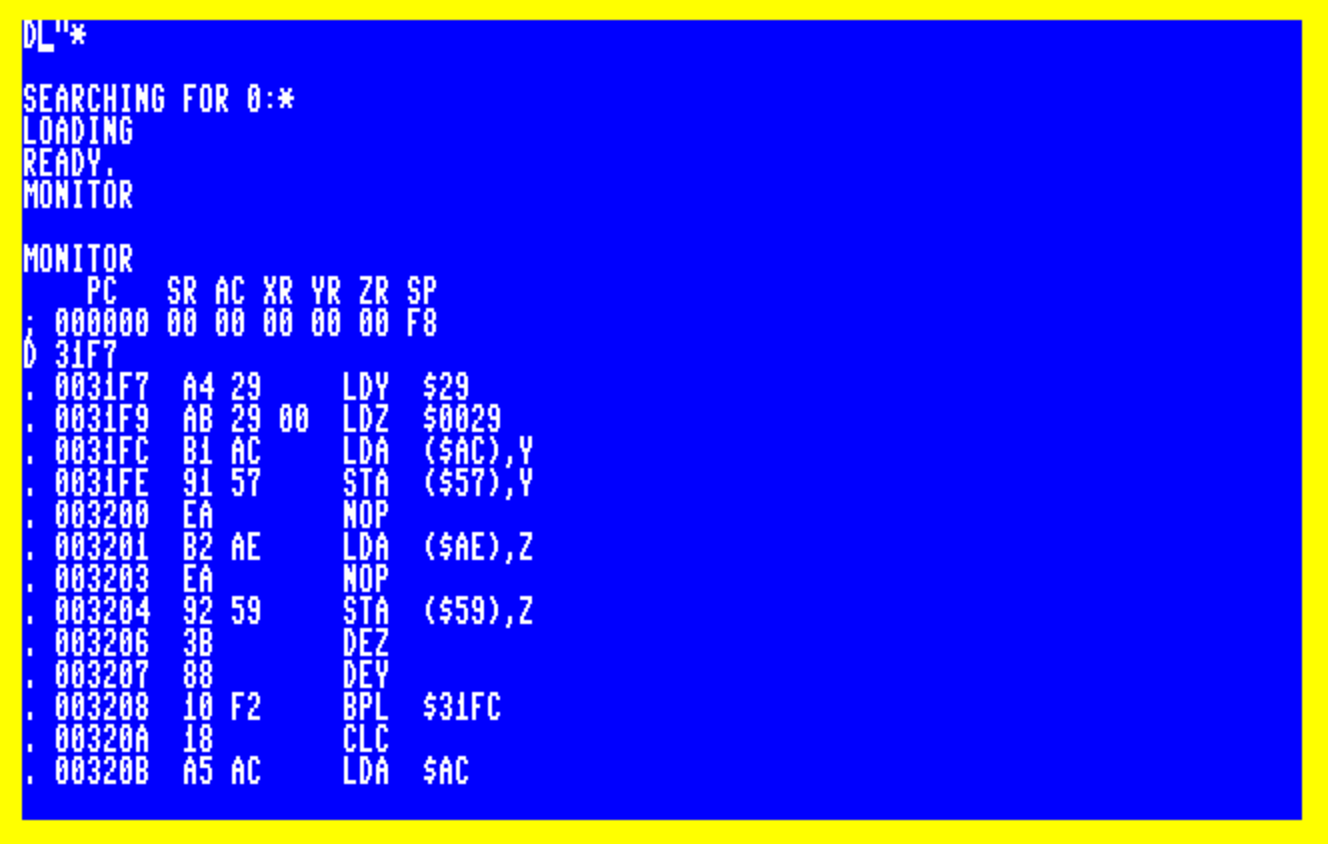
\includegraphics[width=\linewidth]{images/monitor-d}

% ******
% MEMORY
% ******

\subsubsection{M : MEMORY}
\index{MEMORY}
\index{MONITOR Commands!MEMORY}
\begin{description}[leftmargin=2cm,style=nextline]
\item [Format:] {\bf M [from [,to]]}
\item [Usage:] Prints a memory dump for the given address range.
               The dump displays memory contents, organized in rows
               of 16 consecutive addresses starting with the
               address, given as 1st. argument. The dump continues
               until a row has been printed, containing the value
               of the address given as 2nd. argument.
               If no 2nd. argument is present, the dump displays
               a full page of 256 bytes in 16 rows.
               The contents are printed as 16 byte values in hex,
               followed by the character representation.

\item [Remarks:] The rows start with the character '>'.
                 This enables direct full screen editing of the dump.
                 Typing return in any row will write the changed
                 values of the cursor row back to memory, if writable RAM is there.
                 See monitor command {\bf >}.

\item [Example:] Using {\bf M}
\end{description}

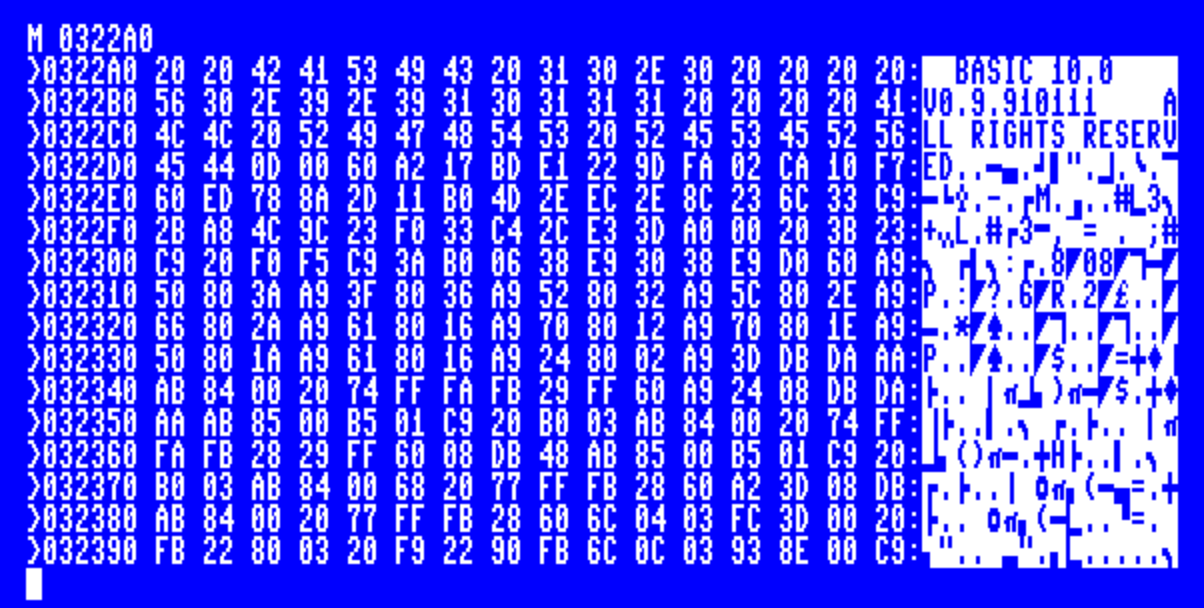
\includegraphics[width=\linewidth]{images/monitor-m}

\section{OpenROMs Enhanced Machine Language Monitor}

This machine language monitor takes the place of the standard C65
machine language monitor. It can be installed by using either an
appropriate version of the OpenROMs, by patching a standard C65 ROM,
or by installing the {\tt MONITOR.M65} file on the SD card of your
MEGA65 (this also requires that you have a sufficiently recent version
of the core support this).

XXX - Document here

\subsection {Calling the Monitor}

To enter the monitor from BASIC, type:
\screentext{MONITOR}

The monitor responds with a display of register contents and waits for a command:

\begin{tcolorbox}[colback=blue,coltext=white]
\verbatimfont{\codefont}
\begin{verbatim}
MONITOR
\end{verbatim}
\begin{tcolorbox}[colback=yellow,coltext=blue,,arc=0mm,boxrule=0mm,
       left*=0.5mm,right*=0mm,top=0mm,bottom=0mm,nobeforeafter,
       left skip=0.1mm,
       width=50mm,height=3mm,valign=center]
\begin{verbatim}
BS MONITOR COMMANDS:ABCDFGHJMRTX@.>;?$+&%'LSV
\end{verbatim}
\end{tcolorbox}
\begin{verbatim}
    PC   SR AC XR YR ZR BP  SP  NVEBDIZC
; 00CFA4 35 00 00 00 00 00 01F8 --11-1-1
\end{verbatim}
\end{tcolorbox}

\subsection{addresses and numbers}

All addresses and numbers must be numbers of base 16 (hex),
10 (decimal), 8 (octal) or 2 (dual). Symbolic names like CHROUT
or arithmetics like \$1000+5 are not allowed.

It is an old tradition since the first monitor of the Commodore PET,
that the default base is 16. In fact the old monitors would not
accept any other numbers, than hexadecimal (short hex).
This may confuse beginners, because a statement like
\begin{verbatim}
LDA #10
\end{verbatim}
loads the decimal value 16 into the accumulator.
Later monitors, like that of the Commodore 128 accepted numbers of
base 16,10,8 and 2 - like this one, but still used 16 (hex) as default.
Additionally the MEGA65 monitor allows character entry, which uses
the PETSCII value of the character.
Following prefixes can be used to specify the base of the following number:

{\ttfamily
{\setlength{\tabcolsep}{1mm}
\begin{tabular}{|l|l|l|l|l|}
\hline
 base  & name & prefix & digits characters & example     \\
\hline
16 & hexadecimal  & \$  & 0123456789ABCDEF & \$100       \\
10 & decimal      &  +  & 0123456789       & +256        \\
 8 & octal        & \&  & 01234567         & \&400       \\
 2 & dual         & \%  & 01               & \%100000000 \\
   & character    &  '  & all              & 'A          \\
\hline
\end{tabular}
}
}

\section{MEGA65 Matrix Mode Monitor Interface}

This monitor is different to the other two: It is part of the MEGA65
system itself, and runs concurrently with MEGA65's processor. That is,
you can view and modify the memory the MEGA65, {\em while a programme is running}.

This works using dedicated hardware in the MEGA65 design, that implements a little
helper processor that runs this monitor interface, and has a special access mechanism
to the memory and processor of the MEGA65.

\subsection {Calling the Monitor}

To enter or exit the monitor hold down the \megasymbolkey and press the \specialkey{TAB} key.
You will see an animation of green characters raining down from the top of the screen, and
then be presented with a simple text terminal interface which is transparent, so that you can
see the screen output of your running programme at the same time.

XXX - Document all commands
